\documentclass[11pt]{article}
\usepackage[margin=0.9in]{geometry}
\usepackage{graphicx}
\usepackage{xcolor}
\usepackage{parskip}
\usepackage{hyperref}
\hypersetup{colorlinks=true, urlcolor=blue, linkcolor=black, citecolor=black}

\definecolor{accent}{RGB}{0,84,140}
\newcommand{\lead}[1]{\textbf{\textcolor{accent}{#1}}\hspace{0.4em}}

%% Headline numbers written by make_exhibits.do; fallback lets this compile
%% before the Stata pipeline has been run.
\IfFileExists{figures/results_macros.tex}{% Auto-generated by make_exhibits.do -- do not edit by hand.
\newcommand{\resNyears}{6}
\newcommand{\resMinYear}{2019}
\newcommand{\resMaxYear}{2024}
\newcommand{\resArrestsTotal}{204,156}
\newcommand{\resArrestsAnnual}{34,026}
\newcommand{\resPolicyCost}{997,215}
\newcommand{\resBenefitBase}{1,455,795}
\newcommand{\resBenefitMid}{3,513,035}
\newcommand{\resNetBase}{458,580}
\newcommand{\resNetMid}{2,515,820}
\newcommand{\resBcrBase}{1.5}
\newcommand{\resBcrMid}{3.5}
\newcommand{\resCostMar}{1,551}
\newcommand{\resCostCoc}{3,440}
\newcommand{\resCostSyn}{1,663}
\newcommand{\resCostOth}{2,603}
\newcommand{\resCostMarFP}{57}
\newcommand{\resPctTests}{49.9}
}{}
\providecommand{\resPolicyCost}{997,772}

\providecommand{\resPolicyCostRounded}{1 million}

\pagenumbering{gobble}

\begin{document}

\begin{center}
    {\LARGE\bfseries The Cost and Benefit of NC HB\,868}\\[4pt]
    {Duke University Economics Analytics Laboratory\footnote{For policy and replication details, please see our attached methodology document.}}
\end{center}

\vspace{4pt}
\hrule
\vspace{10pt}

Roadside colorimetric drug tests are cheap, ubiquitous, and unreliable. The Quattrone Center's review of field drug testing, \emph{Guilty Until Proven Innocent}, documents that these \$2 chemical reagent kits have false positive rates that routinely furnish the probable cause for arrest, booking, and even guilty pleas. Using historical North Carolina arrest data, reports of the costs and likelihood of various judicial outcomes, and North Carolina disposition statistics, we find that:
\begin{itemize}
    \item Under our most conservative estimates, \textbf{the state wastes an average of \$1.5 million on judicial costs by using colorimetric tests.}
    \item When we moderate our assumptions and allow for average judicial costs and progression through the criminal justice system, we find that colorimetrics waste upwards of \$3.5 million
\end{itemize}

\textbf{These costs only account for direct expenses to the state}, and do not account for private costs like lost wages or the social costs of arresting the innocent for drug-related crimes they did not commit.

As an alternative to colorimetric testing that does not decrease North Carolina's capacity to test for drugs, we propose police departments test all potential drugs seized in an arrest using a more reliable test during the booking process, releasing arrestees if the test is negative.\footnote{This proposal is quite similar to the testing reform Colorado adopted in 2026.} We anticipate that this policy would cost roughly \$\resPolicyCostRounded{} per year.


\begin{figure}[h]
  \centering
  \IfFileExists{figures/costbenefit_timeseries.png}{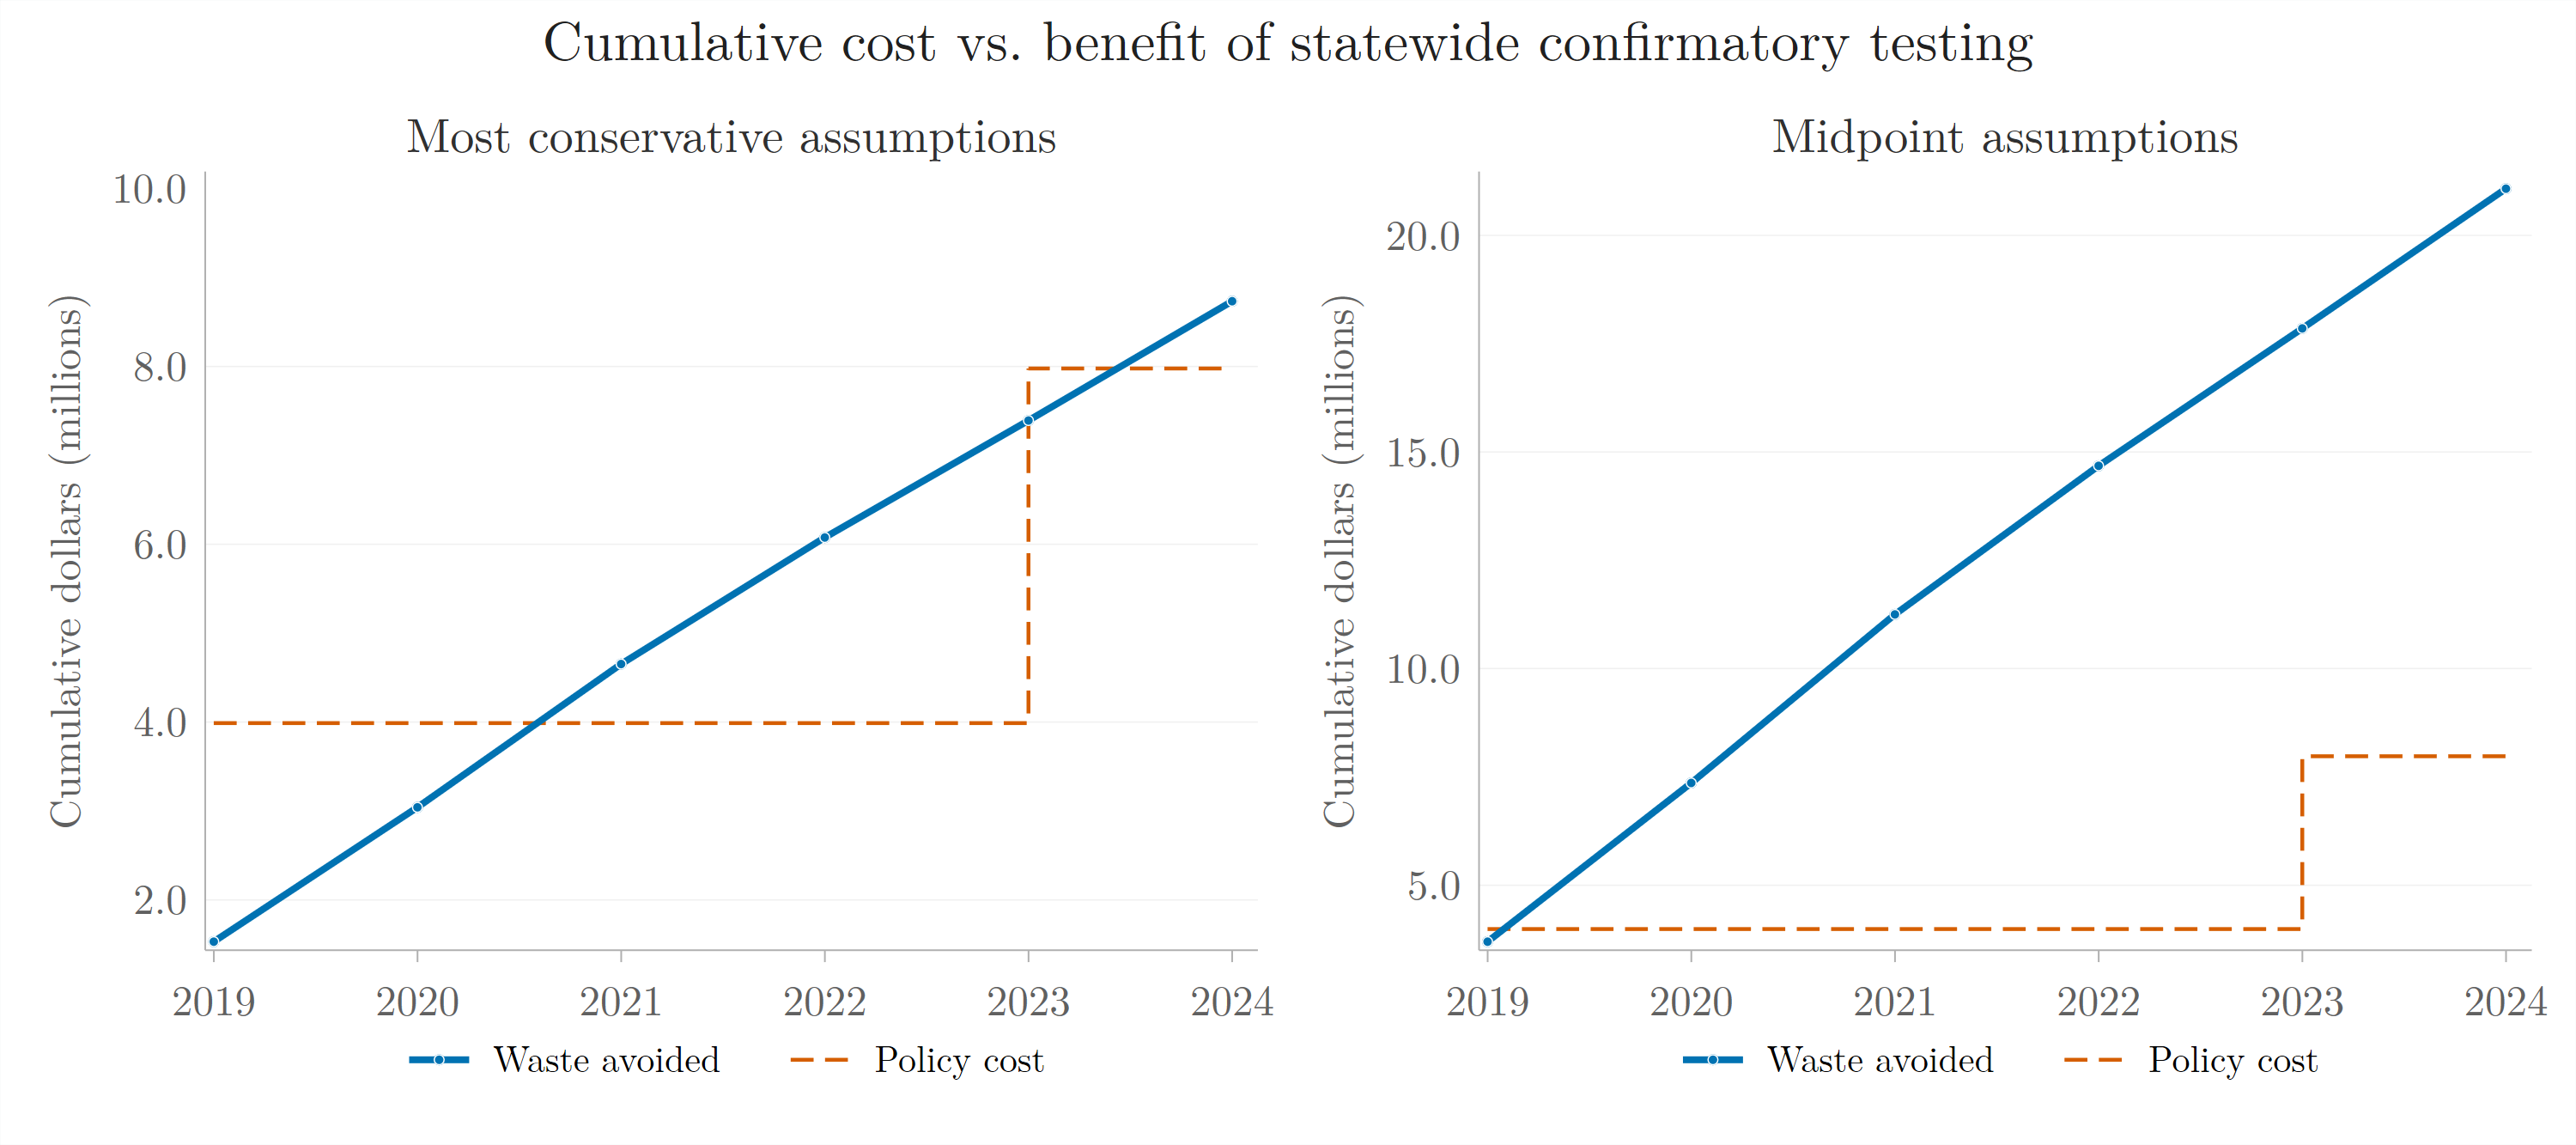
\includegraphics[width=\linewidth]{figures/costbenefit_timeseries.png}}{\textit{[run the Stata pipeline to generate this figure]}}
\end{figure}

We model the effect of enacting this policy in 2019---tracking both savings (blue) and the cost of purchasing and continuously repurchasing the requisite equipment for North Carolina police departments (red dashed). \textbf{Even under our most conservative assumptions, our policy proposal under HB 868 saves a minimum of \$500,000 every year} and breaks even within three years of enactment, even when only accounting for strictly public economic costs

\end{document}
